\section{Ausgabe von Drehmomentverläufen}

Damit die Drehmomente der Antriebe in der Simulation ausgegeben werden können, muss die \en{Actuator Torque}-Variable des jeweiligen \en{Revolute Joint} aktiviert werden. 
Die Variable ist im Bereich \en{Sensing} zu finden, wie Abbildung \ref{fig:simscape_revolute_joint_checkbox} zeigt.
Auf Abbildung \ref{fig:simscape_revolute_joint_block} ist der entsprechende Simscape Block mit aktivierter \en{Actuator Torque}-Variable zu sehen.
\noindent
\\[3cm]
\vspace{-3cm}

\begin{figure}
	\centering
	\begin{subfigure}[b]{0.5\textwidth}
		\centering
		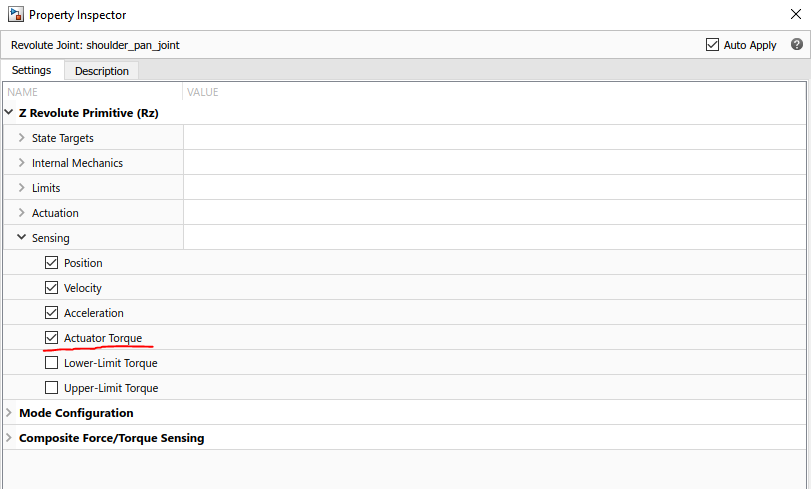
\includegraphics[width=1.0\linewidth]{grafic/actuator_torque}
	\caption{Property Inspector des \en{Revolute Joint}-Blocks mit \en{Actuator Torque}-Checkbox}
	\label{fig:simscape_revolute_joint_checkbox}
	\end{subfigure}
	\begin{subfigure}[b]{0.39\textwidth}
		\centering
		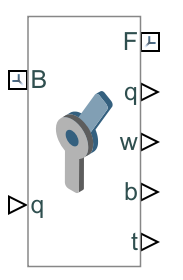
\includegraphics[width=0.3\linewidth]{grafic/revolute_joint}
		\caption{Revolute Joint Simscape Block mit aktivierter \en{Actuator Torque}-Variable}
		\label{fig:simscape_revolute_joint_block}
	\end{subfigure}
	\caption{\en{Property Inspector} des \en{Revolute Joint} und Simscape Block}
\end{figure}

\vspace{2cm}

Danach werden die Ausgaben der Drehmomente aller Gelenke mit dem \en{BusCreator} verbunden, welcher in Abbildung \ref{fig:simulink_logging} auf der linken Seite dargestellt ist.
Die Daten werden dann durch die \en{Log Signals}-Funktion von MATLAB eingeloggt.

\begin{figure}[!htbp]
	\centering
	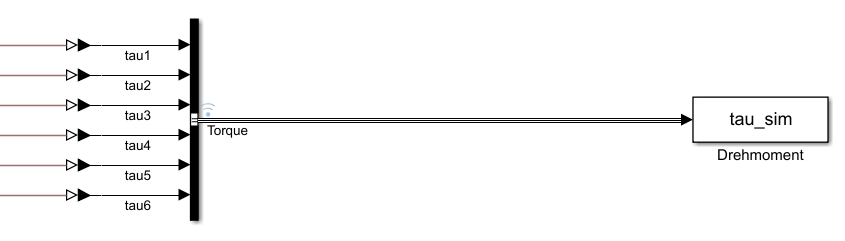
\includegraphics[width=0.8\linewidth]{grafic/torque_busline}
	\caption{Torque Bus Line and Log Sign}
	\label{fig:simulink_logging}
\end{figure}

Die Ergebnisse können im \en{Data Inspector} (Abbildung \ref{fig:drehmomente_simulation}) eingesehen werden.

\begin{figure}[!htbp]
	\centering
	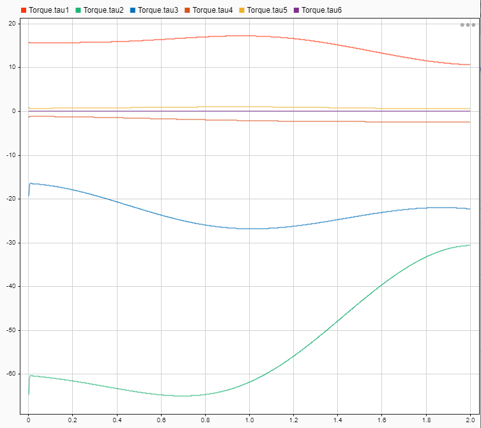
\includegraphics[width=0.5\linewidth]{grafic/Drehmomente}
	\caption{Ausgabe der Drehmomente im \en{Data Inspector}}
	\label{fig:drehmomente_simulation}
\end{figure}

